\chapter{Vers les bases de données graphe}
\label{ch:graph-db}

\section*{Introduction}
\addcontentsline{toc}{section}{Introduction} \markboth{INTRODUCTION}{}

Avec le développement rapide et continu de l'\textit{Internet} et le
\textit{cloud computing}, divers types d'applications ont émergés, ce
qui augmente l'importance accrue de la technologie de base de données,
notamment dans les aspects suivants \cite{han2011survey}:

\begin{itemize}\renewcommand\labelitemi{--}
\item Haute concurrente de lecture et d'écriture avec une faible
  latence.

\item Stockage et la gestion d'une grande masse de données \emph{(Big
    Data)}.

\item Haute scalabilité (évolutivité) et disponibilité.\medskip
\end{itemize}
\enddescription

Bien que les bases de données relationnelles ont occupé une grande
position dans le domaine de stockage de données, le modèle relationnel
commençait à montrer ses limites en faisant face aux plusieurs
exigences: \cite{han2011survey}: lente lecture et l'écriture, capacité
limitée, difficulté d'expansion et scalabilité, etc. Afin de faire
face aux limitations ci-dessus, une variété de nouveaux types de bases
de données ont été apparus qui s'affranchissent du modèle relationnel
pour miser sur le partitionnement horizontal et le relâchement des
contraintes d'intégrité, ce modèle émergent est appelé le modèle
\acrshort{nosql}.\medskip

Dans ce chapitre, nous exposons les différentes approches et
plateformes du stockage \acrshort{nosql} les plus connues dans
l'industrie tout en mettant l'accent sur les bases de données graphes
(et \emph{Neo4j} particulièrement). Nous commençons d'abord par
présenter les quatre catégories majeurs des systèmes
\acrshort{nosql}. Ensuite, nous focalisons sur les \acrshort{SGBD}
orientés graphes, leurs différents modèles et implémentations ainsi
que les langages de requêtes les plus adoptés pour les interroger.

\section{L'environnement NoSQL}
\label{sec:nosql}
\acrshort{nosql} désigne une nouvelle génération de technologies de
gestion de base de données conçu pour répondre à l'augmentation du
volume de données stockées, traitées at analysées par les entreprises
et organisations ayant une large étendue d'utilisateurs tels que
Google Amazon, Facebook et Twitter, \acrshort{nosql} comprend une
multitude de systèmes de gestion de données qui ne sont plus fondés
sur l'architecture classique des bases relationnelles. L'unité logique
n'y est plus la table, et les données ne sont en général pas
manipulées avec \textsc{SQL}.  D'après Fowler \textit{et al.}
\cite{sadalage2012nosql}, Les caractéristiques communes des bases de
données \acrshort{nosql} sont:

\begin{itemize}\renewcommand\labelitemi{--}
\item Ne sont pas fondées sur de le modèle relationnel classique.
\item Optimisées pour les environnements distribués.
\item Construites pour les applications Web modernes avec une grande
  masse de données.
\item \emph{Schemaless} (il n'existe plus d'intégrité référentielle ou
  schéma prédéfini).
\end{itemize}
  \subsection{Catégories des bases de données NoSQL}
  \label{sec:cat-nosql}
  Il existe dans la mouvance \acrshort{nosql} une diversité importante
  d'approches que nous classons en quatre grandes catégories
  \cite{sadalage2012nosql}: dépôts \textit {clés/valeurs}, bases
  orientées documents, orientées colonnes, et bases orientées
  graphes.\bigskip

  \textsf{Dépôts clés/valeurs}: Le principe des bases
  \textit{clé/valeur} est de stocker les données sous une forme
  simple: une \emph{clé } (chaîne de caractères) associé à une
  \emph{valeur} d'une forme libre (chaîne de caractère, ou bien un
  objet sérialisé), cette clé est utilisée pour toutes les opérations
  à effectuer sur les données telles que l'insertion, la mise à jour
  et la suppression. Bien que la structure est plus simple, la vitesse
  d'interrogation est extrêmement supérieur à la base de données
  relationnelles favorisant la scalabilité (\emph{scalability}) plus
  que la cohérence, on les retrouve très souvent comme système de
  stockage de cache ou de sessions distribuées, notamment là où
  l'intégrité relationnelle des données est non significative. Les
  solutions les plus connues, telles que \emph{Redis}, \emph{Riak} et
  \emph{Voldemort} sont principalement influencés par le projet
  \emph{Dynamo} d'Amazon \cite{decandia2007dynamo}.\bigskip

  \textsf{Orientées documents}: Cette famille de base de données est
  une évolution de la base de données \textit{clé/valeur} destinée aux
  applications qui gèrent des documents (généralement du format
  \textsc{JSON} ou \textsc{XML}) où chaque clé n'est plus associée à
  une valeur sous forme de bloc binaire mais à un document dont la
  structure reste libre (\textit{scheme-less}). L'avantage est de
  pouvoir récupérer, via une seule clé, un ensemble d’informations
  structurées de manière hiérarchique. ainsi que le stockage de
  volumes très importants de données pour lesquelles la modélisation
  relationnelle aurait entraînée une limitation des possibilités de
  partitionnement et de réplication. les deux implémentations les plus
  populaires dans cette catégorie sont \emph{CouchDB} d'Apache et
  \emph{MongoDB}.\bigskip

  \textsf{Orientées colonnes}: La famille des stockages orientés
  colonnes sont une évolution du modèle \textit{clé/valeur} utilisant
  des \textit{``familles''} afin de grouper certaines lignes. Ces
  familles peuvent devenir hiérarchiques et les relations entre les
  données deviennent explicites. Une base de données orientées
  colonnes permet de plus une compression par colonne, efficace
  lorsque les données de la colonne se ressemblent. Comme solutions,
  on retrouve principalement \emph{HBase}, \emph{HyperTable}
  (implémentations Open Source du modèle \emph{BigTable}
  \cite{chang2008bigtable} publié par Google) ainsi que
  \emph{Cassandra} (projet Apache qui respecte l'architecture
  distribuée de \emph{Dynamo} \cite{decandia2007dynamo} d'Amazon et le
  modèle BigTable de Google).\bigskip

  \textsf{Orientées graphes}: Ce paradigme est le moins connu de ceux
  de la mouvance \acrshort{nosql}. Ce modèle s'appuie principalement
  sur deux concepts: d'une part l'utilisation d'un moteur de stockage
  pour les objets (qui se présentent sous la forme d'une base
  documentaire, chaque entité de cette base étant nommée
  \emph{nœud}). D'autre part, à ce modèle, vient s'ajouter un
  mécanisme permettant de décrire les relations entre les objets
  (\emph{arcs}). Principalement, ces bases de données sont nettement
  plus efficaces que leur pendant relationnel pour traiter les
  problématiques liées aux réseaux.  En effet, lorsqu'on utilise le
  modèle relationnel, cela nécessite un grand nombre d'opérations
  complexes (souvent, des jointures trop lentes) pour obtenir des
  résultats. Dans cette catégorie on peut citer \emph{Neo4j},
  \emph{OrientDB}, \emph{Titan} et \emph{AllegroGraph} comme les
  implémentations les plus répondus de ce modèle.

  \subsection{Le théorème de CAP }
  \label{sec:cap}
  \acrshort{cap} \cite{brewer2000towards} est l'acronyme de
  \textit{``\textbf{C}onsistency, \textbf{A}vailability and
    \textbf{P}artition Tolerance''}, ou \textit{``Cohérence,
    Disponibilité et Résistance au partitionnement''}. Ce théorème
  explique qu'il est impossible qu'un système distribué satisfasse
  simultanément aux trois contraintes suivantes:\medskip

  \begin{figure}[h]
    \centering
    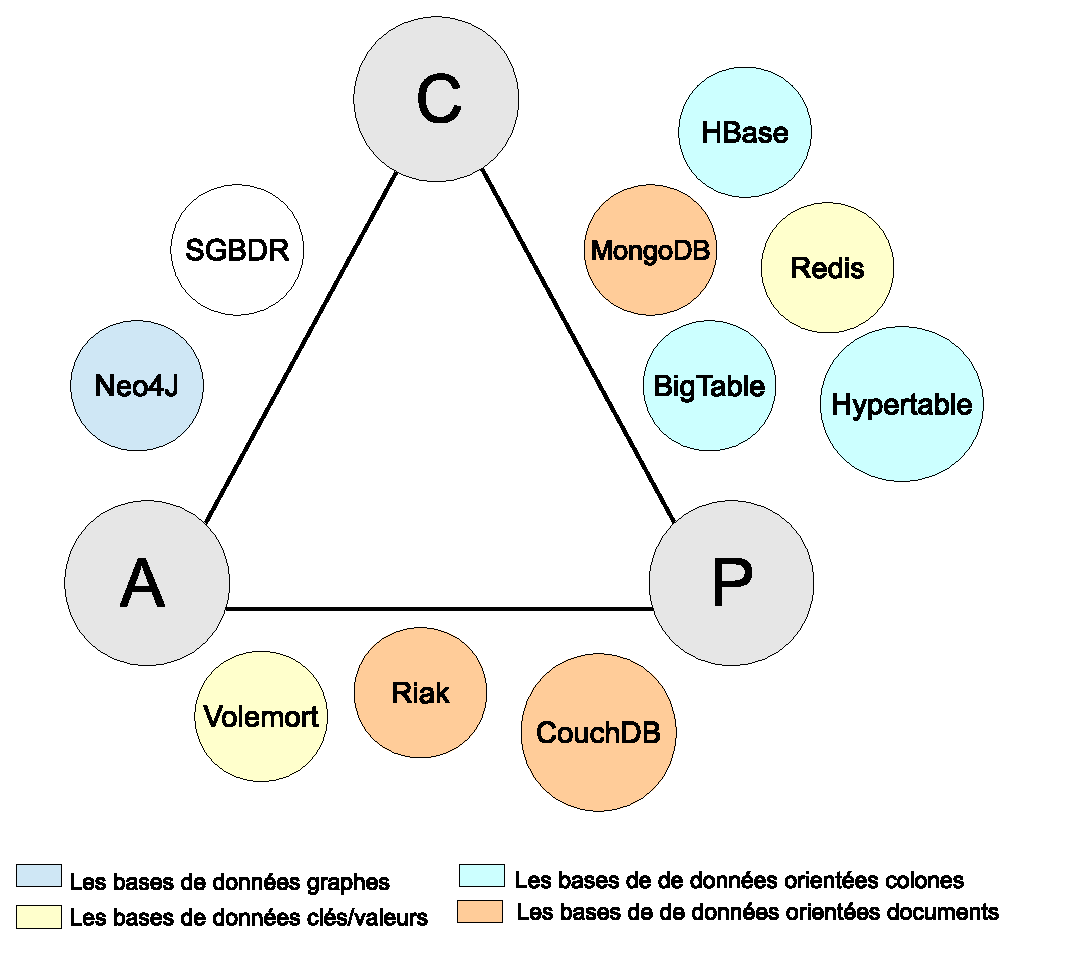
\includegraphics[width=0.96\textwidth]{figs/cap.eps}
    \caption{Le théorème CAP}
    \label{fig:cap}
\end{figure}

%%% Local Variables:
%%% mode: latex
%%% TeX-master: "../main"
%%% End:


  \renewcommand{\descriptionlabel}[1]{\hspace{0.5cm}\textbullet~\textsf{#1}}
  \begin{description}
  \item [Cohérence]: tous les nœuds du système voient exactement les
    mêmes données au même moment.

  \item [Disponibilité]: la perte de nœuds n'empêche pas les survivants
    de continuer à fonctionner correctement.

  \item [Résistance au partitionnement]: aucune panne moins importante
    qu'une coupure totale du réseau ne doit empêcher le système de
    répondre correctement.\medskip
  \end{description}
  \enddescription


  Le théorème de \acrshort{cap} stipule qu'il est impossible d'obtenir
  ces trois propriétés en même temps dans un système distribué et
  qu'il faut donc en choisir deux parmi les trois, Les bases de
  données relationnelles implémentent les propriétés de cohérence et
  de disponibilité (système \emph{CA}). Les bases de données
  \emph{NoSQL} sont généralement des systèmes \emph{CP} (cohérent et
  résistant au partitionnement) ou \emph{AP} (disponible et résistant
  au partitionnement), la figure \ref{fig:cap} présente le
  positionnement de quelque systèmes \emph{NoSQL} par rapport au
  théorème \acrshort{cap}.

\section{Bases de données orientées graphes}
\label{sec:graph-database-overview}
Cette section a pour but d'introduire les modèles de données utilisés
pour la persistance la persistance et la gestion d'un graphe de
données fortement connectées \ref{sec:persistence}, ainsi que les
techniques du stockage sous-jacent et d'indexation utilisées par les
différents systèmes de gestion de base de données graphes.
\ref{sec:graph-internals}.\medskip

\subsection{Définitions et caractéristiques}
\label{sec:graphdb-defs}

Un grand nombre de problèmes pratiques dans différentes disciplines
peuvent être intuitivement représentés sous forme de graphes (des
nœuds reliés par des arcs ou des arêtes).\medskip

Depuis plusieurs décennies, les développeurs ont essayé de stocker des
ensembles de données connectés, \textit{semi-structurées} à
l'intérieur des bases de données relationnelles. Mais alors que les
bases de données relationnelles ont été initialement conçues pour
codifier des structures tabulaires. Cependant, les données fortement
connectées sont traitées de manière très pauvre par les bases de
données relationnelles. Chaque opération sur une relation dans un
graphes ou réseau résulte en une opération de jointure dans le
\acrshort{SGBDR}. Implémentées comme des opérations ensemblistes entre
l'ensemble des clés primaires de deux tables, les jointures sont des
opérations lentes et sans capacité à monter en charge alors que le
nombre de tuples de ces tables augmente
\cite{robinson2013graph}.\medskip


Angles Gutierrez \cite{angles2008survey} proposent une définition:

% \renewcommand{\descriptionlabel}[1]{\hspace{0.5cm}\textbullet~\textsf{#1}}
% \begin{description}
% \item [Data and/or the schema]
% \item [Data manipulation]
% \item [Integrity constraints]
% \end{description}
% \enddescription

% "Une base de données graphe brille quand elle stocke des données
% hautement " "connectées.  Les requêtes sont exécutées à l'aide de
% traversées, qui peuvent " "procéder à plusieurs millions de
% traversées par seconde.  Une traversée " "ressemble à une _jointure_
% dans les bases de données relationnelles.


% Une base de données graphe stocke les données en graphe, structure de
% " "données la plus générique, capable de représenter avec élégance
% n'importe " "quel type de données d'une manière ultra
% accessible


% Les bases de données orientées graphes sont donc conçues pour
% modéliser des réseaux de données fortement connectées et y naviguer
% facilement en bénéficiant de performances extrêmement élevées\medskip

  \subsection{Techniques de persistance des bases de données graphes}
  \label{sec:persistence}
  Généralement, nous pouvons distinguer trois techniques majeures du
  stockage adoptés par les systèmes de gestion des bases de données
  graphes: les bases de données graphes qui utilisent des
  \acrshort{SGBDR} comme un \emph{backend}, celles qui utilisent des
  systèmes \acrshort{nosql}, et enfin, nous avons les bases de données
  graphes natives qui fournissent ses propres implémentations du
  stockage en termes des nœuds et des arcs directement.

    \newpage
    \subsubsection{Bases de données graphes au-dessus de d'un stockage  SQL}
    \label{sec:graphdb-over-sql}
    Une base de donnée graphe peut être stockée dans une base de
    données relationnelle. Les étiquettes et les attributs de nœuds et
    arcs peuvent être gérés séparément dans d'autres tables et renvoyé
    par des clés étrangères. l'utilisation des \acrshort{SGBDR} comme
    un moteur de stockage a quelques avantages : des systèmes
    d'indexation évolués, un support des transactions sophistiqué, et
    le langage de requêtes \emph{SQL} qui est un standard bien établi
    avec a cycle d'apprentissage rapide.\medskip

    \begin{figure}[h]
    \centering
    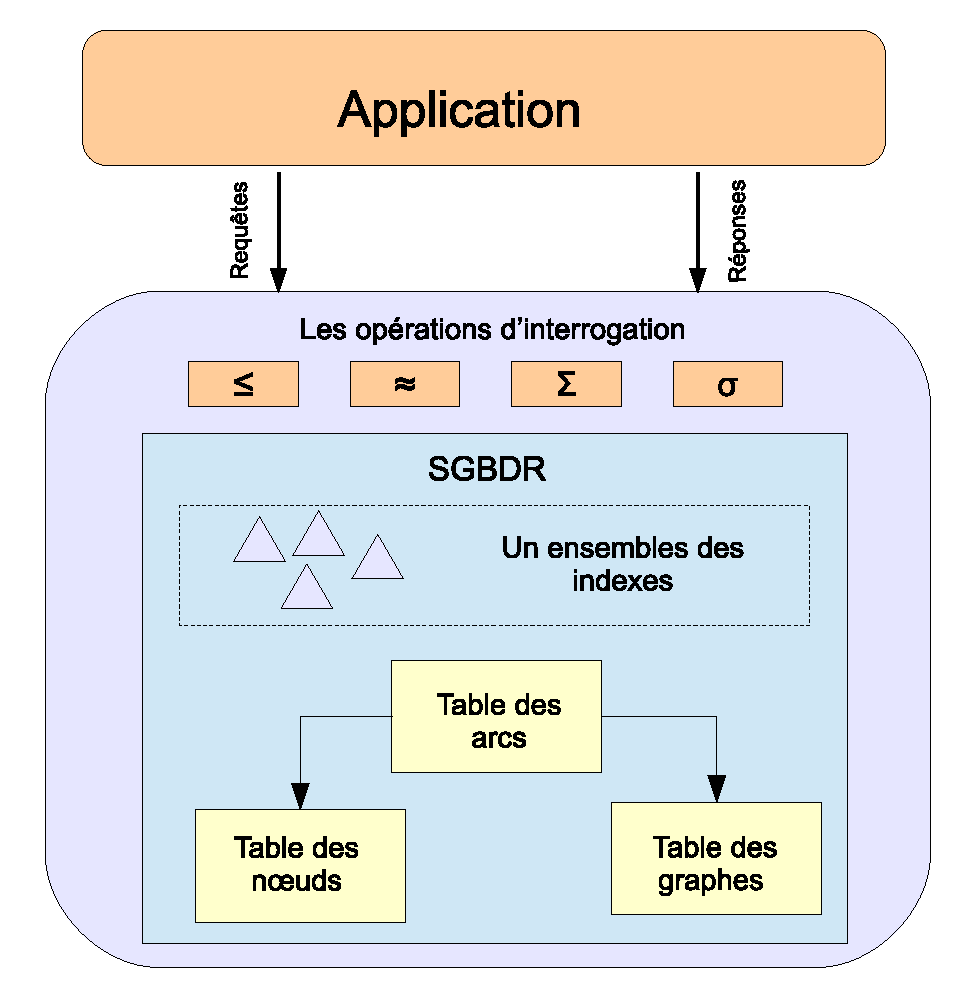
\includegraphics[width=0.8\textwidth]{figs/periscope-gq.eps}
    \caption{L'architecture du système Periscope/GQ \cite{tian2008periscope}}
    \label{fig:periscope-gq}
\end{figure}

%%% Local Variables:
%%% mode: latex
%%% TeX-master: "../main"
%%% End:


    Cette classe comprend \emph{GRIPP} \cite{trissl2007fast}, et
    Periscope/GQ \cite{tian2008periscope} développé par l'université
    de Michigan qui implémente un système de gestion des bases de
    données graphes comme une application au-dessus d'un moteur de
    stockage relationnel \emph{PostgreSQL}.


    \subsubsection{Bases de données graphes au-dessus d'un stockage NoSQL}
    \label{sec:graphdb-over-nosql}
    Plusieurs systèmes de base de données graphes emploient des
    systèmes \acrshort{nosql} comme un moteur de stockage interne
    offrant une meilleure scalabilité et un support fiable pour le
    partitionnement des données.\bigskip

    \textsf{HypergraphDB} \cite{hypergraphdb,
      iordanov2010hypergraphdb} est une base de donnée qui implémente
    le modèle de données \emph{``hypergraph''} où la notion d'un arc
    est étendue pour pouvoir connecter plus de deux nœuds, ce qui est
    particulièrement utile pour la modélisation des données tels que
    la représentation des connaissances, l'intelligence artificielle
    et la bio-informatique. \emph{HypergraphDB} utilise le modèle
    \textit{clé/valeur} de \emph{BerkeleyDB} \cite{berkeleydb} pour
    stocker toutes les informations relatives du graphe sous forme de
    pairs \textit{clé/valeur}, chaque objet du graphe (nœud ou arc)
    est identifié par un clé unique (appelé atome). Chaque atome est
    lié à un ensemble des atomes par une relation de type \emph{0:N}
    (zéro ou plusieurs atomes), ces relations forment également la
    structure typologique ``hypergraph''.\bigskip

    \textsf{OrientDB} \cite{orientdb} est un système hybride de
    gestion de base de données graphes qui combine les fonctionnalités
    d'une base orientée documents et une base orientée graphes avec
    une capacité de stockage des données structurées ou
    semi-structurées (\emph{schema-less}). il supporte aussi la
    répartition de charge à travers plusieurs machines et la
    réplication multi-maîtres tout en assurant les propriétés
    \acrshort{acid} de données. Pour les requêtes simples,
    \emph{OrientDB} s'appuie sur \emph{SQL} et utilise des langages de
    parcours des graphes comme \emph{Gremlin} afin d'éviter les
    jointures \emph{SQL} coûteuses pour les requêtes
    complexes.\bigskip

    \textsf{Titan} \cite{titan} est une base de données orientée
    graphes évolutive (\emph{scalable}) et transactionnelle, optimisée
    pour le stockage et l'interrogation des données graphes contenant
    des centaines de milliards de sommets et d'arcs à travers un
    \emph{cluster} multi-machine avec des schémas complexes du
    parcours et requêtage et une exécution en temps réal. \emph{Titan}
    utilise une multitude des systèmes \emph{NoSQL} comme un moteur de
    stockage (\emph{backend}), par exemple, \emph{Hbase},
    \emph{Cassandra}, \emph{BerkeleyDB}, cette diversité offre une
    flexibilité en terme des caractéristiques \emph{CAP} \ref{sec:cap}
    assurées par le système.

    \subsubsection{Les bases de données graphes natives}
    \label{sec:graphdb-native}
    Les bases de données graphes natives possèdent leurs propres
    systèmes de fichiers pour stocker les données au lieu de compter
    sur des moteurs de stockage tiers. Ces bases de données sont
    optimisés pour stocker et gérer les données \textbf{fortement}
    connectées où la performance et la disponibilité sont
    primordiales.\bigskip

    % TODO: enhance
    \textsf{Neo4j} \cite{neo4j} est un système de gestion de base de
    données graphes \textit{open-source} populaire implémenté en
    \textit{java} et supporté commercialement par \textit{Neo
      Technology}\footnote{\url{http://neo4j.com/}}. il a été
    conceptualisé et construit depuis le début afin d'être un système
    fiable, robuste, évolutif et très performant optimisé pour stocker
    et gérer des grandes masses de données structurées en graphe,
    \textit{Neo4j} convient aussi bien pour le deploiement en grande
    entreprise que pour les projets plus légers en utilisant une
    partie du serveur complet. Parmi ses fonctionnalités:\medskip

    \begin{itemize}\renewcommand\labelitemi{--}
    \item Transactions \acrshort{acid} réelle avec unr haute disponibilité.
    \item Supporte jusqu'à des milliards de noeuds et relations.
    \item Requêtes ultra-rapides grâce aux traversées.
    \end{itemize}
    \enddescription
    \medskip

    \textit{Neo4j} est fourni avec une \textit{API} basée sur des
    \textit{callbacks}, ce qui vous laisse la possibilité de spécifier
    les règles pour les traversées, Les autres options pour traverser
    ou interroger un graphe dans \textit{Neo4j} sont \textit{Gremlin}
    \ref{sec:gremlin} et \textit{Cypher} \ref{sec:cypher}.\bigskip

    \textsf{AllegroGraph} \cite{allegrograph} est un système performant
    de persistance des données graphes avec un stockage natif,
    implémenté initialement comme une système de persistance et
    gestion de documents \acrshort{rdf} doté d'un interface
    \acrshort{rest} \cite{fielding2000architectural}. Similaire à
    \emph{Neo4j}, \emph{Allegrograph} garantis la satisfaction des
    propriétés \acrshort{acid} d'atomicité, cohérence, isolation et
    durabilité. \emph{AllegroGraph} supporte \acrshort{sparql}, RDFS++
    et \textit{Prolog} pour des applications clientes
    multiples.\bigskip

    \textsf{Sparsity} \cite{sparksee} (auparavant connu sous le nom
    \emph{DEX}) est un système natif de stockage de données graphes
    persistants et temporaires. \emph{Sparsity} focalise sur la
    gestion et l'interrogation des géantes bases de données graphes à
    haute performance. En encodant les matrices d'adjacences en
    \emph{bitmap}, le système a une gestion d'espace disque compact et
    efficace afin de d'assurer une très bonne performance.\medskip
    \newpage

    \textsf{InfiniteGraph} \cite{infinitegraph} est un système
    distribué de gestion des bases de données graphes qui supporte des
    grandes masses évolutives de données (\emph{large-scale}) avec une
    capacité d'analyse efficace des graphes et une bonne prise en
    charge des algorithmes distribués du
    parcours. \emph{InfiniteGraph} fournis une variété
    d'implémentations pour des différents systèmes (serveurs
    d'application, les plateformes de \emph{cloud computing} et les
    systèmes embarqués).

  \subsection{Techniques de stockage et d'indexation}
  \label{sec:graph-internals}
  Il ya plusieurs façons représenter un graphe dans une mémoire
  principale d'un système de stockage. On dit qu'un système de gestion
  des base de données graphes dispose des capacités \emph{natives} de
  parcours des graphes s'il est possède une propriété fondamentale
  appelée \emph{index-free adjacency}.

  \begin{figure}[!hr]
    \centering
    \begin{subfigure}[h]{0.7\textwidth}
        \centering
        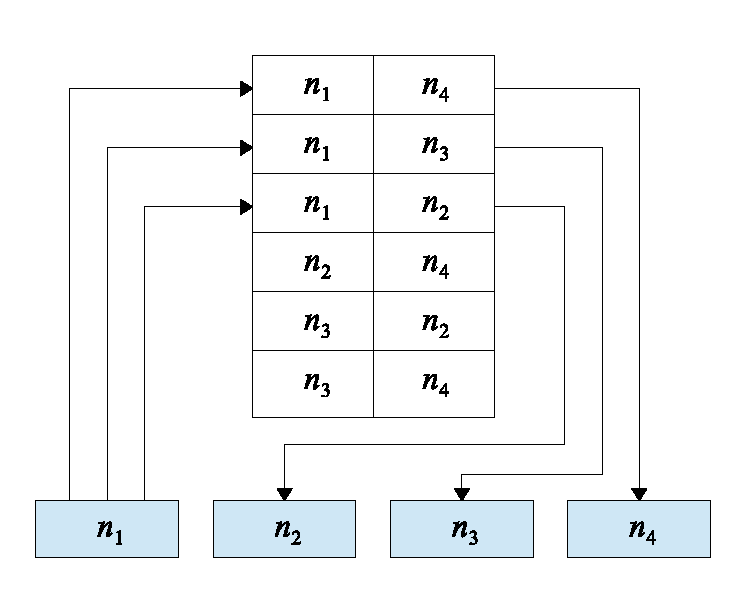
\includegraphics[width=\textwidth]{figs/global-graph-index-table.eps}
        \label{fig:global-graph-index-table}
    \end{subfigure}

    \begin{subfigure}[h]{0.45\textwidth}
        \centering
        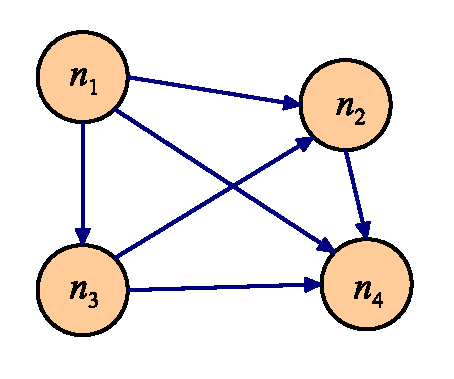
\includegraphics[width=\textwidth]{figs/global-graph-index.eps}
        \label{fig:global-graph-index}
    \end{subfigure}

    \caption{Une indexation global des données fortement connectées}
    \label{fig:gpi}
\end{figure}

%%% Local Variables:
%%% mode: latex
%%% TeX-master: "../main"
%%% End:

  \newpage

    \subsubsection{Index-free adjacency}
    \label{sec:index-free}
    Dans un système de stockage de base de données graphes qui utilise
    la technique \emph{index-free adjacency}, chaque noeud maintient
    des références directs à ses noeuds adjacents agissant comme un
    micro index d'autres noeuds voisins. Cette méthode améliore la
    fiabilité du système de stockage d'une façon considérable
    comparant à cels qui utilise un index global. En effet, le temps
    de réponse des requêtes est indépendant à la taille globale du
    graphe. Pour traverser une graphe d'une taille donnée $n$ à $m$
    pas, le coût est d'ordre $\mathcal{O}(m\log{}n)$ dans un système
    avec un index globale, et d'ordre $\mathcal{O}(m)$ pour un système
    natif qui utilise un \emph{index-free adjacency}.

    \begin{figure}[h]
    \centering
    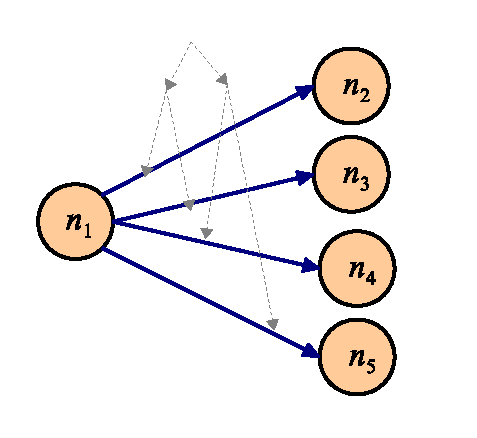
\includegraphics[width=0.5\textwidth]{figs/vertex-centric-indices.eps}
    \caption{Vertex centric indices}
    \label{fig:vertex-centric-indices}
\end{figure}
%%% Local Variables:
%%% mode: latex
%%% TeX-master: "../main"
%%% End:


    \subsubsection{Vertex Centric Indices}
    \label{sec:vertex}        % TODO: enhance the vertex stuff ...

    Vertex Centric Indices (\emph{Titan} \cite{vertexci}): L'objectif
    de cette technique est de trier et indexer tous arcs incidents
    d'un noeud (et donc les noeud adjacents) selon les propriétés de
    ces arcs. Ces indexes éliminent la nécessité de balayage linéaire
    des arcs incidents lors d'un requête de parcours
    ($\mathcal{O}(n)$) en faveur d'un parcours plus rapide (
    $\mathcal{O}(n)$ ou $\mathcal{O}(\log{}n)$). Cette méthode est
    utilisée surtout pour confronter le problème de \emph{Supernode}
    dans les graphes fortement connectés, un \emph{Supernode} est un
    noeud avec un très grand nombre des arcs incidents.

  % \newpage
  % \subsection{Comparaison}
  % \label{sec:graphdb-comp}
  % \begin{table}[htb!]
  \centering
  \begin{tabular}{|lcccc|}
  \end{tabular}
  \newline
  \caption{Comparaison des bases de données graphes}
  \label{tab:graphdb-comp}
\end{table}

%%% Local Variables:
%%% mode: latex
%%% TeX-master: "../main"
%%% End:

  % \newpage

  % {\color{red}
  %   to be continued
  % }
  % \newpage

\section{Langages des requêtes}
\label{sec:query-languages}
Les langages de requêtes ont toujours été la clé du succès des
\acrshort{SGBD}. La prévalence des \emph{\acrshort{SGBDR}} dans les
dernières décennies est étroitement couplée avec le succès du
\emph{SQL}. Des divers langages ont été définis pour exprimer des
requêtes vis-à-vis plusieurs dépôts de données, par exemple,
\emph{XQuery} \cite{boag2002xquery} et \emph{XPath}
\cite{clark1999xml} pour les bases de données \emph{\acrshort{xml}},
\emph{QQL} \cite{alashqur1989oql} pour les bases de données orientées
objets et \acrshort{sparql} \cite{prud2008sparql} pour les
triplestores (les bases de données \emph{RDF}).

\begin{figure}[!h]
  \centering
  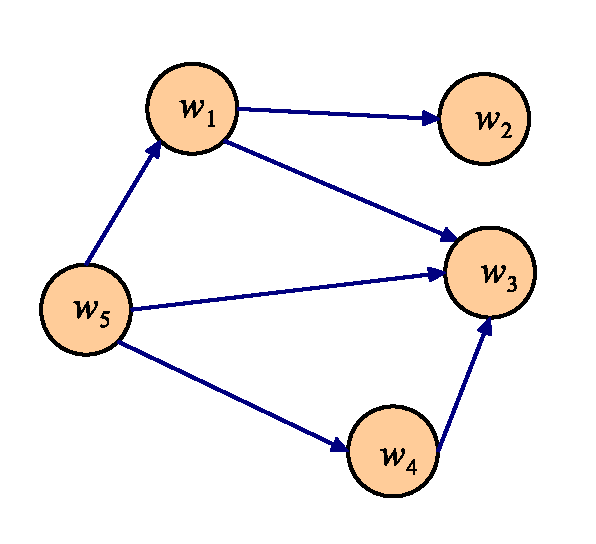
\includegraphics[width=0.6\textwidth]{figs/query-graph-example.eps}
  \caption{Un example d'un graphe orienté}
  \label{fig:query-graph-example}
\end{figure}

%%% Local Variables:
%%% mode: latex
%%% TeX-master: "../main"
%%% End:


Cette section présente trois langages de requêtes largement supportés
par les systèmes de gestion des bases de données graphes. Le graphe
présenté par la figure \ref{fig:query-graph-example} sera utilisé pour
illustrer le syntaxe et la sémantiques de ces trois langages. Le
graphe représente le résultat d'un processus de \emph{matching}
sémantique entre cinq service Web qui forme un plan de composition.


  % definition
  % example
  % syntax
  % graph-db support
\newpage
  \subsection{SPARQL}
  \label{sec:sparql}

  \acrshort{sparql} \cite{prud2008sparql} est un langage populaire de
  requêtes pour les données \acrshort{rdf}, il est reconnu comme l'une
  des technologies clés du Web sémantique. Le standard
  \acrshort{sparql} est largement utilisé pour exprimer des
  interrogations à travers diverses sources de données graphes vues
  comme des triplestores \acrshort{rdf}. Il est capable de rechercher
  des motifs de graphe (\emph{graph patterns}) ainsi que leurs
  conjonctions et leurs disjonctions. Les résultats des interrogations
  \acrshort{sparql} peuvent être des ensembles de résultats ou des
  graphes \acrshort{rdf} qui peuvent être retournés via
  \acrshort{http} dans une variété de formats tels que \acrshort{xml},
  HTML ou \acrshort{json}\medskip

  % TODO:approve!
  \acrshort{sparql} propose quatre types de requêtes:\medskip

  \begin{itemize}\renewcommand\labelitemi{--}
  \item les requêtes \texttt{SELECT} permettent d'extraire des
    informations d'une base de données ou d'une source de données
    \acrshort{rdf} interrogée.
  \item les requêtes \texttt{CONSTRUCT} permettent de créer de
    nouveaux triplets à partir du résultat d'une requête.

  \item les requêtes \texttt{DESCRIBE} permettent d'obtenir la
    description d'une ressource donnée. Les spécifications de
    \acrshort{sparql} ne précisent pas la nature de la description
    d'une ressource. Elles imposent seulement que cette description
    soit un sous-ensemble du graphe interrogé.

  \item les \texttt{ASK} retournent un booléen indiquant si la requête
    à une solution ou n'en a pas.
  \end{itemize}
  \enddescription
  \medskip

  La plupart des bases de données graphes ont un support de
  \textsc{SPARQL} soit nativement telle que \emph{Allegrograph} soit
  via des extensions comme dans le cas de \emph{Neo4j}.
  \newpage

  \subsection{Gremlin}
  \label{sec:gremlin}
  \emph{Gremlin} \cite{gremlin-wiki} est un langage de domaine
  spécifique (\acrshort{DSL}) de bas niveau pour le parcours des
  graphes attribués, il trouve ses applications dans les domaines de
  la recherche, l'analyse et la manipulation des bases de données
  orientées graphes qui implémentent le modèle \emph{Blueprints}
  \cite{blueprints} de données. \emph{Gremlin} \cite{gremlin-wiki} est
  un projet open source développé et maintenu par
  \emph{TinkerPop}.\medskip

  Le syntaxe \emph{Gremlin} est basée sur \emph{XPath} de manière à
  être capable d'exprimer des descriptions de parcours même profonds
  avec des expressions simples et compactes.\medskip

  La distribution \emph{Gremlin} (maintenu par \emph{TinkerPop}) est
  supporté par la plupart des bases de données graphes via des
  langages \emph{JVM} comme \emph{Java}, \emph{Groovy} et
  \emph{Scala}, parmi ces \acrshort{SGBD} graphes nous trouvons
  \emph{Neo4j}, \emph{Titan} et \emph{OrientDB}.

  \newpage
  \subsection{Cypher}
  \label{sec:cypher}
  \emph{Cypher} \cite{cypher-docs} est un langage des requêtes
  déclaratif pour interagir avec les bases des données graphes
  \emph{Neo4j}, développé et maintenu par \emph{Neo Technology}. Il
  permet d'effectuer des requêtes et mises jour du graphe efficaces
  sans avoir écrire de traversiers (parcours) d'une manière
  procédurale.\medskip

  En étant un langage déclaratif, \emph{Cypher} se concentre sur la
  clarté d'exprimer \textit{quoi retrouver dans un graphe et non
    comment le faire}. Ceci est en contraste aux langages impératifs
  comme Java et aux langages script comme \emph{Gremlin}
  \ref{sec:gremlin}, ce qui rend le fait d'optimisation de requêtes un
  détail d'implémentation non exposé aux utilisateurs. \emph{Cypher}
  est inspiré de plusieurs approches et construit sur des pratiques
  établies pour l'interrogation expressif des bases de données. La
  plupart des mots clés comme \verb|WHERE| et \verb|ORDER BY|, et La
  concordance de patterns sont hérités directement des langages
  déclaratifs comme \emph{SQL} et \emph{SPARQL} \ref{sec:sparql} avec
  quelque propriétés inspirés des langages fonctionnels comme
  \emph{Haskell} et \emph{ML}.\medskip

  Le langage \emph{Cypher} comporte un nombre de clauses distinctes,
  des clauses pour l'interrogation du graphe comme:
  \begin{itemize}
  \item [\texttt{MATCH}]: Utilisé pour pour décrire Le pattern du graphe
    à correspondre, principalement sur la base de relations entre les
    nœuds du graphe.
  \item [\texttt{WHERE}]: Sert à un critère de filtrage.
  \item [\texttt{RETURN}]: Spécifie ce qu'il faut retourner comme
    résultat finale de requête.
  \end{itemize}
  \medskip

  \emph{Cypher} contient en outre des clauses pour l'écriture, la mise
  à jour et suppression de données, par exemple:

  \begin{itemize}
  \item [\texttt{CREATE}]: Crée des nœuds ou des relations.
  \item [\texttt{SET}]: Affecte des valeurs aux propriétés..
  \item [\texttt{DELETE}]: supprime des noeuds, relations ou propriétés.
  \end{itemize}

  \newpage

\section*{Conclusion}
\label{sec:conclusion}
\addcontentsline{toc}{section}{Conclusion} \markboth{CONCLUSION}{}

%%% Local Variables:
%%% mode: latex
%%% TeX-master: "../main"
%%% End:
